\documentclass[letterpaper, 10pt, conference]{ieeeconf}
\IEEEoverridecommandlockouts \overrideIEEEmargins
\usepackage{amsmath,amssymb,url,times,subfigure,graphicx,theorem}
\usepackage{graphicx,subfigure,hyperref}
\usepackage{color,comment}
\usepackage{csquotes}
%\usepackage{refcheck}

\usepackage{epic,eepic}

\usepackage[]{algorithm2e}
%\usepackage{algorithmicx}
%\usepackage{algpseudocode}

%\usepackage{algorithm}
%\usepackage{algpseudocode}
%\usepackage{pifont}



%\usepackage{amsmath}
%\usepackage{algorithm}
%\usepackage[noend]{algpseudocode}
%
%\makeatletter
%\def\BState{\State\hskip-\ALG@thistlm}
%\makeatother



\newcommand{\norm}[1]{\ensuremath{\left\| #1 \right\|}}
\newcommand{\abs}[1]{\ensuremath{\left| #1 \right|}}
\newcommand{\bracket}[1]{\ensuremath{\left[ #1 \right]}}
\newcommand{\braces}[1]{\ensuremath{\left\{ #1 \right\}}}
\newcommand{\parenth}[1]{\ensuremath{\left( #1 \right)}}
\newcommand{\ip}[1]{\ensuremath{\langle #1 \rangle}}
\newcommand{\refeqn}[1]{(\ref{eqn:#1})}
\newcommand{\reffig}[1]{Fig. \ref{fig:#1}}
\newcommand{\tr}[1]{\mbox{tr}\ensuremath{\negthickspace\bracket{#1}}}
\newcommand{\trs}[1]{\mbox{tr}\ensuremath{\!\bracket{#1}}}
\newcommand{\deriv}[2]{\ensuremath{\frac{\partial #1}{\partial #2}}}
\newcommand{\G}{\ensuremath{\mathsf{G}}}
\newcommand{\SO}{\ensuremath{\mathsf{SO(3)}}}
\newcommand{\T}{\ensuremath{\mathsf{T}}}
\renewcommand{\L}{\ensuremath{\mathsf{L}}}
\newcommand{\so}{\ensuremath{\mathfrak{so}(3)}}
\newcommand{\SE}{\ensuremath{\mathsf{SE(3)}}}
\newcommand{\se}{\ensuremath{\mathfrak{se}(3)}}
\renewcommand{\Re}{\ensuremath{\mathbb{R}}}
\newcommand{\Sph}{\ensuremath{\mathsf{S}}}
\newcommand{\aSE}[2]{\ensuremath{\begin{bmatrix}#1&#2\\0&1\end{bmatrix}}}
\newcommand{\ase}[2]{\ensuremath{\begin{bmatrix}#1&#2\\0&0\end{bmatrix}}}
\newcommand{\D}{\ensuremath{\mathbf{D}}}
\renewcommand{\d}{\ensuremath{\mathbf{d}}}
\newcommand{\pair}[1]{\ensuremath{\left\langle #1 \right\rangle}}
\newcommand{\met}[1]{\ensuremath{\langle\!\langle #1 \rangle\!\rangle}}
\newcommand{\Ad}{\ensuremath{\mathrm{Ad}}}
\newcommand{\ad}{\ensuremath{\mathrm{ad}}}
\newcommand{\g}{\ensuremath{\mathfrak{g}}}

\title{\LARGE \bf
Bayesian Occupancy Grid Mapping via Exact Inverse Sensor Model}

\author{Evan Kaufman, Taeyoung Lee%
\thanks{Evan Kaufman, Taeyoung Lee, Mechanical and Aerospace Engineering, George Washington University, Washington DC 20052 {\tt \{evankaufman,tylee\}@gwu.edu}}
\thanks{This research has been supported in part by NRL under the grant *********, and NSF under the grants CMMI-1243000, CMMI-1335008, and CNS-1337722.}
}


\newcommand{\EditTL}[1]{{\color{red}\protect #1}}
%\renewcommand{\EditTL}[1]{{\protect #1}}


\newtheorem{definition}{Definition}
\newtheorem{lem}{Lemma}
\newtheorem{prop}{Proposition}
\newtheorem{cor}{Corollary}
\newtheorem{remark}{Remark}



\begin{document}
\allowdisplaybreaks


\maketitle \thispagestyle{empty} \pagestyle{empty}

\begin{abstract}
Occupancy grid maps are spatial representations of environments, where the space of interest is decomposed into a number of cells that are considered either occupied or free. This paper is focused on occupancy grid mapping, which is to estimate the probability of occupancy for each cell based on range measurements from a known location. For a given probabilistic model of a range sensor, we propose a computationally efficient method to obtain an exact inverse sensor model, and it is utilized to construct a probabilisitic mapping algorithm according to the Bayesian framework. Compared with the existing occupancy grid mapping techniques that rely on approximate inverse sensor models, the proposed approach yields substantially more accurate maps for the same set of measurements. These are illustrated by numerical examples and experiments. 
\end{abstract}

\section{Introduction}

Mapping in the context of robotics is to generate a representation of the environment around the robot.
This problem is crucial to understanding the surrounding regions when a robot enters an uncertain environment
Various map representations have been applied to the mapping problem such as occupancy grids~\cite{WolSuk05}, octomaps~\cite{WurHorBenStaBur10}, or with distinguishable features in a landmark representation~\cite{MonThrKolWeg02}.
To build maps in real time, a computationally-efficient algorithm is required.% \EditTL{rewrite this paragraph for mapping, without introducing SLAM here}

This paper focusses on the popular occupancy grid representation, where the map space is decomposed into evenly-spaced grid cells that are considered as either occupied or free. Obtaining the probability of occupancy for a grid cell based on range measurements and the configuration of the mobile robot, known as the \emph{inverse sensor model}, is of fundamental importance with occupancy grid mapping. However, the exact solution to the inverse sensor model has not been utilized in occupancy grid mapping, because the computational requirements appear too cumbersome to compute the exact model in real time~\cite{ThrBurFox05}.

Instead, several techniques have been proposed to approximate the exact inverse sensor model. %Due to the computational limitations, two common approaches are applied to obtain a function close to the inverse sensor model.
In the early occupancy grid mappings based on sonar sensors, \emph{ad hoc} techniques are employed to obtain an inverse sensor model, where the bearings of depth measurements are considered uncertain because the directions of bouncing sound waves are highly inaccurate~\cite{MorElf85,Elf89}.
%These occupancy grid mapping schemes employ \emph{ad hoc} techniques to obtain the inverse sensor model.
These techniques are based on approximate functions to represent the inverse sensor model with questionable accuracy~\cite{ChoLynHutKanBurKavThr05} and applied to more modern sensors in~\cite{And09},~\cite{PirRutBisSch11}.

The other popular approach to obtain an approximate inverse sensor model is to simulate maps, robot poses, and measurements and use a learning algorithm, such as neural network to approximate the inverse sensor model~\cite{Thr01,ThrBurFox05}. These approaches are undesirable in practice due to complexities associated to implementing a learning algorithm. For example, the accuracy of such inverse sensor models strongly depends on the samples selected for learning, but it is unclear how to select those samples or how many samples are required to obtain a reasonable approximation. Furthermore, it is challenging to apply any learning algorithm over the large dimensional space composed of maps, poses, and measurements. 

%and they only yield probabilistic approximations without strong mathematical justification. 

%These approaches simply treat occlusions with discrete probabilities of detection, regardless of whether one cell may completely, partially, or not block another cell in the sensor field of view.

%Furthermore, both approaches follow a log-odds ratio Bayesian framework, imposing an additional Markov assumption.

%These techniques are not also suitable for modern range sensor with the highly accurate bearing~\cite{Thr03}. Based on recent improvements in sensor technology, the occupancy grid mapping problem has been restructured using the fact that depth measurement bearings are known. \EditTL{do we need this paragraph?}

This paper proposes a computationally efficient algorithm to construct the exact inverse sensor model. More explicitly, for a given forward sensor model defined by the probability distribution of range measurements, this algorithm yields a posteriori probability of occupancy of all of the cells within the area covered by the range sensor from the range measurements. The key idea is reducing the computational load by using the fact that if a cell is occupied, the occupancy of the other cells blocked by it is irrelevant to the forward sensor model, and it is systematically utilized with various probabilistic properties to derive a computationally-efficient solution to the inverse sensor model. Furthermore, the proposed approach integrates a priori probability of occupancy and multiple range measurements according to the Bayesian framework to obtain more accurate maps. As such, it is contrast to the existing framework based on log-odds ratios that impose an additional Markov assumption. 

%these are constructed 

In short, the main contribution of this paper is proposing the exact inverse sensor model and utilizing it into Bayesian occupancy grid mapping. Compared with the current mapping algorithms based on an approximate inverse sensor model, this approach yields more accurate occupancy probabilities. This constructs substantially more accurate occupancy grid maps with less uncertainty for the same set of measurements, and these are directly illustrated by numerical examples and preliminary experimental results. While this paper is focused on the mapping problem in the two-dimensional environments, the presented results can be certainly utilized in SLAM or stochastic motion planning in three dimensions.


%occupancy probabilities that are more accurate than prior work, which may be applied for more accurate real-time map generation in the SLAM problem and more effective trajectory planning strategies based on map uncertainty.

The paper is organized as follows.
The problem is formulated in Section \ref{sec:ProbForm}, and the exact solution to the occupancy grid mapping problem is derived in Section \ref{sec:ISM}.
A numerical result shows the improved accuracy in Section \ref{sec:NumRes}, and an experimental result with the Kinect depth sensor shows the improvement in map certainty in Section \ref{sec:ExpRes}, followed by conclusions.


\section{Problem Formulation}
\label{sec:ProbForm}

\subsection{Range Sensor}

Consider a range sensor that provides scans of surrounding maps to identify the closest occupied space. The location and the direction of the sensor, referred to as \emph{pose} at time $t$ is denoted by $X_t$. The range sensor returns a measurement \emph{scan} $Z_t$, which is composed of $n_z$ measurement \emph{rays} $z_{t,1},z_{t,2},...,z_{t,n_z}$. The $l$-th measurement ray for $l\in\braces{1,2,...,n_z}$ contains the depth (range) and bearing (direction) of a small region inside the sensor field of view (FOV) that corresponds to a circular sector.

The probability density function, namely $p(z_{t,l}|m,X_t)$ with respect to depth of the $l$-th measurement ray conditioned on the map $m$ and the pose $X_t$ is commonly referred to as a \emph{forward sensor model}, which characterizes the corresponding depth sensor, such as the maximum range or accuracy. The forward sensor model satisfies  ($i$) the ranges of all depth measurements are positive and finite, and ($ii$) measurement rays cannot pass through occupied regions.

Throughout this paper, it is assumed that the forward sensor model of the selected sensor is given. This can be determined empirically or analytically. For example, the \emph{beam model for range finders} satisfying  the above criteria is described in~\cite{ThrBurFox05}.
%, which contains Gaussian, exponential, uniform, and point pass portions~\cite{ThrBurFox05}.
%At time $t$ and given the pose $X_t$ and map $m$, the beam model with respect to the $l$-th measurement ray $z_{t,l}$ is the probability density defined as
%\begin{align}
%p(z_{t,l})=\begin{cases}
%\frac1{z_{max}-z_{min}}P_{hit}+P_{short}+P_{rand}\ \text{if},\ 
%\\
%P_{max},
%\end{cases}
%\end{align}
%where $z_{min}\leq z_{t,l}\leq z_{max}$ and $\hat z_{t,l}$ is the distance between the robot and the closest occupied location along the direction $z_{t,l}$.
%The probabilities are defined such that $P_{hit}$ is the probability of the depth originating from this occupied location (Gaussian), $P_{exp}$ is the probability that an unexpected occlusion blocks the first occupied location of the map (exponential), $P_{rand}$ is the probability of a phantom reading (uniform), and $P_{max}$ is the probability that the sensor returns its maximum value (point mass).
%These probabilities are normalized such that
%\begin{align}
%P_{hit}+P_{short}+P_{rand}+P_{max}=1.
%\end{align}

%We assume that this forward sensor model depends on the closest occupied location, and is independent of the occupancy beyond this point.
	
\subsection{Occupancy Grid Mapping}

Let a map $m$ be decomposed into $n_m$ evenly-spaced grid cells, where the $i$-th grid cell is assigned to a static binary random variable $\mathbf{m}_i$ for $i\in\braces{1,2,...,n_m}$, that is defined as $\mathbf{m}_i=1$ when it is occupied, and $\mathbf{m}_i=0$ when it is free. Another binary random variable is defined as $\bar{\mathbf{m}}_i=1-\mathbf{m}_i$ for convenience.
Therefore, the probability that the $i$-th cell is occupied is $P(\mathbf{m}_i)$, and the probability that it is free is $P(\bar{\mathbf{m}}_i)=1-P(\mathbf{m}_i)$. The location and size of each grid cell are assumed to be known.
%, but its occupancy is uncertain; the occupancy is treated as a binary random variable such that $P(\mathbf{m}_i)$ is the probability that $\mathbf{m}_i$ is occupied and $P(\bar{\mathbf{m}}_i)$ is the probability that $\mathbf{m}_i$ is free, such that $P(\mathbf{m}_i)+P(\bar{\mathbf{m}}_i)=1$.
The occupancies of different cells are assumed independent such that
\begin{align}
P(m)=P(\mathbf{m}_1,\mathbf{m}_2,...,\mathbf{m}_{n_m})=\prod_{i=1}^{n_m}P(\mathbf{m}_i).
\end{align}

%Occupancy grid mapping produces a probabilistic map; none of the $n_m$ grid cell occupancies are completely certain.
Note that there are $2^{n_{m}}$ possible maps. The occupancy grid mapping problem is to determine these probabilities based on robot poses, measurement scans, and the forward sensor model. More explicitly, let $X_{1:t}$ denotes the history of poses from the initial time to the current time, $\{X_1,X_2,\ldots, X_t\}$, and let $Z_{1:t}$ be the measurement history. Therefore, the goal is to obtain $P(\mathbf{m}_i|X_{1:t},Z_{1:t})$, commonly referred to as the \emph{inverse sensor model}, for all grid cells.

	% Def of occupancy grid
	% Cell occupancies are assumed independent
	% Probabilistic maps
	% Notations
	% Mapping problem
	
\subsection{Mapping via Log-Odds Ratio}

One of the popular frameworks of updating binary random variables with static state is with a binary Bayesian filter using the log-odds ratio formulation.
The main idea is that instead of multiplying terms from prior and current time steps, the properties of logarithms allow these terms to be simply added, while avoiding truncation issues associated with probabilities close to $0$ or $1$~\cite{ThrBurFox05}.
The log-odds ratio is also popular because learning techniques with forward models~\cite{Thr01},~\cite{Thr03} or ad hoc techniques~\cite{MorElf85},~\cite{Elf89} are simpler to derive when they need not consider $P(\mathbf{m}_i|X_{1:t},Z_{1:t-1})$ as part of the inverse sensor model, but rather only $P(\mathbf{m}_i)$, which is typically fixed and uniform for all cells.

However, the log-odds ratio formulation makes an assumption that is not consistent with the occupancy grid mapping problem. Early on, the derivation assumes that if $X_t$ and $\mathbf{m}_i$ are known, then $Z_t$ is independent of $X_{1:t-1}$ and $Z_{1:t-1}$, i.e.,
%\begin{align}
%\label{eqn:FirstBayesRule}
%P(\mathbf{m}_i|X_{1:t},Z_{1:t})
%&
%=\frac{P(Z_t|\mathbf{m}_i,X_{1:t},Z_{1:t-1})P(\mathbf{m}_i|X_{1:t},Z_{1:t-1})}{P(Z_t|X_{1:t},Z_{1:t-1})}.
%\end{align}
\begin{align}
\label{eqn:AssumptionEarly}
P(Z_t|\mathbf{m}_i,X_{1:t},Z_{1:t-1})\approx P(Z_t|\mathbf{m}_i,X_t).
\end{align}
The above equation can be justified if both sides are conditioned by the complete map instead of $\mathbf{m}_i$, since the probability distribution of the sensor is completely determined by its pose and the map. However, since it is conditioned only by the $i$-th cell, past poses $X_{1:t-1}$ and past measurement scans $Z_{1:t-1}$ may have certain information about the occupancy of the other cells, which should be considered in calculating the probability distribution of the measurement $Z_t$.  In short, this log-odds framework is based on the assumption that neglects potentially important information contained in $X_{1:t-1}$ and $Z_{1:t-1}$.


%However, past poses $X_{1:t-1}$ and past measurement scans $Z_{1:t-1}$ may suggest that there exist occupied regions that occlude some or all of $Z_t$ from detecting $\mathbf{m}_i$ from the current pose $X_t$.
%Since this assumption neglects potentially important information contained in $X_{1:t-1}$ and $Z_{1:t-1}$, this framework is subject to poor results.
%Hence, the log-odds ratio formulation is completely avoided in further analysis.


	
	% approximated inverse sensor model
	% markov assumption
	% shortcoming, reason this is avoided
	
\section{Exact Inverse Sensor Model}
\label{sec:ISM}

Due to the computational complexity, approximate inverse sensor models have been used for occupancy grid mapping with simplifying assumptions. In this section, we propose an algorithm to compute the exact inverse sensor model efficiently. 
%Much like the forward sensor model that reasons measurements from a known map, he inverse sensor model reasons that map from known measurements~\cite{ThrBurFox05}.
While the inverse sensor model varies slightly in meaning in numerous publications, two versions are derived in this paper, both based on a Bayesian framework.
The first type is referred to as the \emph{ray inverse sensor model} $P(\mathbf{m}_i|X_{1:t},Z_{1:t-1},z_{t,l})$, which only considers $l$-th ray at time $t$.
The second type is referred to as the \emph{scan inverse sensor model} $P(\mathbf{m}_i|X_{1:t},Z_{1:t})$, which combines the information from \emph{all} measurement rays \emph{simultaneously} at the $t$-th time step.


These are contrary to inverse sensor models commonly used with the log-odds ratio formulations, and the proposed algorithm integrates all of past poses and measurement scans with the current ones to obtain more accurate estimate of the map.

\subsection{Ray Inverse Sensor Model}

Suppose the probability of the map conditioned on the past poses and measurements, namely $P(m|X_{1:t-1},Z_{1:t-1})$ are is. Here we construct a posteriori probability $P(m|z_{t,l},X_{1:t},Z_{1:t-1})$, based on the current pose $X_t$, a measurement ray $z_{t,l}$, and the given forward sensor model $p(z_{t_l}|m,X_t)$.

\paragraph{Bayesian Framework}
Assuming that the probability density of the sensor measurement is fixed over a small measurement region $\Delta z$, Bayes' rule yields
%First, Bayes' rule is applied for a particular map $m$ and arbitrarily small measurement region $\Delta z$, yielding
\begin{align}
\label{eqn:BayesRuleRayISM}
P(&m|z_{t,l},X_{1:t},Z_{1:t-1})\nonumber
\\
&=\frac{p(z_{t,l}|m,X_{1:t},Z_{1:t-1})\Delta zP(m|X_{1:t-1},Z_{1:t-1})}{P(z_{t,l}|X_{1:t},Z_{1:t-1})},
\end{align}
where we have used the fact that $X_t$ carries no information about $m$ without $Z_t$.
If the current pose $X_t$ and map $m$ are known, then the measurement ray $z_{t,l}$ is independent of past poses $X_{1:t-1}$ and past measurements $Z_{1:t-1}$.
%Note that this is contrary to approaches that consider $X_t$ and $\mathbf{m}_i$ (not the full map $m$) as enough information, ignoring the occupancy of other cells in this term.
Then, \refeqn{BayesRuleRayISM} can be rewritten as
\begin{align}
P(m|z_{t,l},&X_{1:t},Z_{1:t-1})\nonumber
\\
&
=\eta_{t,l}p(z_{t,l}|m,X_{t})P(m|X_{1:t-1},Z_{1:t-1}),
\end{align}
where the normalizing constant $\eta_{t,l}=\frac{\Delta z}{P(z_{t,l}|X_{1:t},Z_{1:t-1})}\in\Re$ absorbs all terms independent of the map $m$.

%Assuming $z_{t,l}$ measures an occupied cell, then $z_{t,l}$ may be a result of the occupancy of $\mathbf{m}_i$, or $z_{t,l}$ may measure a different occupied cell.

Next, we compute the occupancy probability of each cell. Let $\mathcal{M}_i$ be the set of maps where the $i$-th cell is occupied, i.e., $\mathcal{M}_i =\{m\in\{0,1\}^{2_{n_m}}\,|\ \mathbf{m}_i=1\}$. To compute the probability of occupancy of the $i$-th cell, all possible combinations of map in $\mathcal{M}_i$ should be considered, i.e., 
%All possible combinations of map $m$ must be considered in which $\mathbf{m}_i$ is occupied, denoted as $m:m(i)=\mathbf{m}_i$,
\begin{align}
\label{eqn:InvSenModWithProbDens}
&P(\mathbf{m}_i|z_{t,l},X_{1:t},Z_{1:t-1})\nonumber
\\
&=\eta_{t,l}\sum_{m\in\mathcal{M}_i}p(z_{t,l}|m,X_{t})P(m|X_{1:t-1},Z_{1:t-1}).
\end{align}
Furthermore, to determine the normalizing constant $\eta_{t,l}$, its its complement $P(\bar{\mathbf{m}}_i|z_{t,l},X_{1:t},Z_{1:t-1})$ must be calculated in the similar manner. Since there are $2^{n_{m}-1}$ maps in $\mathcal{M}_i$, it appears that these equations require additions $2^{n_m}$ times for the $i$-th grid cell, and it should be repeated for other cells.
%However, this is not the case when the bearing of $z_{t,l}$ is known. (\EditTL{Not sure why bearing matters})
	
\paragraph{Computationally Efficient Approach}
Define a reduced map $r$ where the $k$-th cell is denoted $\mathbf{r}_k$ such that $k\in\braces{1,2,...,n_r}$ with $n_r\leq n_m$.
This reduced map is chosen such that each cell of $r$ corresponds to a grid cell of $m$ that $z_{t,l}$ intersects, ordered by increasing distance, which is easily determined with geometry.
Then let the term $\mathbf{r}_{k+}$ mean that the $k$-th cell is occupied, cells with lower index are free, and cells with greater index may or may not be occupied; put differently, the $k$-th cell $\mathbf{r}_k$ is the closest occupied cell to current pose $X_t$ along reduced map $r$.
This means that the forward sensor model $p(z_{t,l}|\mathbf{r}_{k+},X_{t})$ depends on the distance from $X_t$ to the $k$-th cell, and \emph{no other cells}.



\begin{prop}
Let the $k$-th unnormalized probability of the inverse sensor model be defined as
\begin{align}
\label{eqn:Unnormalized}
\tilde P(\mathbf{r}_k|z_{t,l},&X_{1:t},Z_{1:t-1})=\frac1{\eta_{t,l}}P(\mathbf{r}_k|z_{t,l},X_{1:t},Z_{1:t-1})\nonumber\\&=P(\mathbf{r}_k|X_{1:t-1},Z_{1:t-1})\nonumber\\
&\quad\times \sum_{i=1}^{k-1}\left\{\prod_{j=0}^{i-1}P(\bar{\mathbf{r}}_j|X_{1:t-1},Z_{1:t-1})\right\}\nonumber\\
&\quad\times p(z_{t,l}|\mathbf{r}_{i+},X_t)P(\mathbf{r}_i|X_{1:t-1},Z_{1:t-1})
%\\
%\label{eqn:UnnormalizedCompl}
%\tilde P(\bar{\mathbf{r}}_k|z_{t,l},X_{1:t},Z_{1:t-1})&=\frac1{\eta_{t,l}}P(\bar{\mathbf{r}}_k|z_{t,l},X_{1:t},Z_{1:t-1})
,
\end{align}
where the normalizer $\eta_{t,l}$ is defined as
\begin{align}
\label{eqn:allEta}
\eta_{t,l}
&=
\bigg[\sum_{i=1}^{n_r}\left\{\prod_{j=0}^{i-1}P(\bar{\mathbf{r}}_j|X_{1:t-1},Z_{1:t-1})\right\}\nonumber\\&\quad\times p(z_{t,l}|\mathbf{r}_{i+},X_t)P(\mathbf{r}_i|X_{1:t-1},Z_{1:t-1})\bigg]^{-1}.
\end{align}


%respectively.
These have the follow solutions that may be obtained in a computationally-efficient manner:
\begin{align}
\label{eqn:tildePresult}
\tilde P(\mathbf{r}_k|z_{t,l},&X_{1:t},Z_{1:t-1})=P(\mathbf{r}_k|X_{1:t-1},Z_{1:t-1})\nonumber\\
&\quad\times \sum_{i=1}^{k-1}\left\{\prod_{j=0}^{i-1}P(\bar{\mathbf{r}}_j|X_{1:t-1},Z_{1:t-1})\right\}\nonumber\\
&\quad\times p(z_{t,l}|\mathbf{r}_{i+},X_t)P(\mathbf{r}_i|X_{1:t-1},Z_{1:t-1})
\nonumber
\\
&\quad
+
\left\{\prod_{j=0}^{k-1}P(\bar{\mathbf{r}}_j|X_{1:t-1},Z_{1:t-1})\right\}\nonumber\\
&\quad\times p(z_{t,l}|\mathbf{r}_{k+},X_t)P(\mathbf{r}_k|X_{1:t-1},Z_{1:t-1}),
\\
\label{eqn:tildePcomplementresult}
\tilde P(\bar{\mathbf{r}}_k|z_{t,l},&X_{1:t},Z_{1:t-1})
=P(\bar{\mathbf{r}}_k|X_{1:t-1},Z_{1:t-1})\nonumber\\
&\quad\times \sum_{i=1}^{k-1}\left\{\prod_{j=0}^{i-1}P(\bar{\mathbf{r}}_j|X_{1:t-1},Z_{1:t-1})\right\}\nonumber\\
&\quad\times p(z_{t,l}|\mathbf{r}_{i+},X_t)P(\mathbf{r}_i|X_{1:t-1},Z_{1:t-1})
\nonumber
\\
&\quad
+
\sum_{i=k+1}^{n_r}\left\{\prod_{j=0}^{i-1}P(\bar{\mathbf{r}}_j|X_{1:t-1},Z_{1:t-1})\right\}\nonumber\\
&\quad\times p(z_{t,l}|\mathbf{r}_{i+},X_t)P(\mathbf{r}_i|X_{1:t-1},Z_{1:t-1}).
\end{align}
\end{prop}
\begin{proof}
See the Appendix 1.
\end{proof}


Because $\mathbf{r}_k$ is binary, the following holds:
\begin{align}
\label{eqn:allEta}
\eta_{t,l}&=\frac1{\tilde P(\mathbf{r}_k|z_{t,l},X_{1:t},Z_{1:t-1})+\tilde P(\bar{\mathbf{r}}_k|z_{t,l},X_{1:t},Z_{1:t-1})}\nonumber
\\
&=
\bigg[\sum_{i=1}^{n_r}\left\{\prod_{j=0}^{i-1}P(\bar{\mathbf{r}}_j|X_{1:t-1},Z_{1:t-1})\right\}\nonumber\\&\quad\times p(z_{t,l}|\mathbf{r}_{i+},X_t)P(\mathbf{r}_i|X_{1:t-1},Z_{1:t-1})\bigg]^{-1},
\end{align}
where $\eta_{t,l}$ is independent of the index $k$ of the reduced map.
Rearranging \refeqn{Unnormalized} and \refeqn{UnnormalizedCompl}, the ray inverse sensor model is 
\begin{align}
\label{eqn:RayISMAnswer}
P(\mathbf{r}_k|z_{t,l},X_{1:t},Z_{1:t-1})&=\eta_{t,l}\tilde P(\mathbf{r}_k|z_{t,l},X_{1:t},Z_{1:t-1}),
\\
P(\bar{\mathbf{r}}_k|z_{t,l},X_{1:t},Z_{1:t-1})&=\eta_{t,l}\tilde P(\bar{\mathbf{r}}_k|z_{t,l},X_{1:t},Z_{1:t-1}),
\end{align}
respectively, where $\eta_{t,l}$ comes from \refeqn{allEta} and the unnormalized probabilities come from \refeqn{tildePresult} and \refeqn{tildePcomplementresult}.

Compared with the ray inverse sensor model described with \refeqn{InvSenModWithProbDens} considering $n_r$ possible cells, where the summation should be repeated $2^{n_r}$ times \emph{per cell of the reduced map}, the proposed expressions  \refeqn{allEta}, \refeqn{tildePresult}, and \refeqn{RayISMAnswer} are \textit{substantially} simpler.
In fact, if the terms inside the summations of \refeqn{tildePresult} are obtained recursively, only $n_r$ repetitions are required for \emph{all cells of the reduced map}, yielding an algorithm that is up to $\mathbf{2^{n_r}}$ \textbf{times faster}.

\subsection{Scan Inverse Sensor Model}

The goal of occupancy grid mapping is to obtain the probabilistic map based on all measurements and poses, including the latest measurement scan.
At the $t$-th time step, the mesauremenet scan is the set of all rays $Z_t=\{z_{t,1},z_{t,2},...,z_{t,n_z}\}$, which serve to update the map occupancy probabilities in a unified way.
\paragraph{Bayesian Framework} Assuming the measurement rays are mutually independent, Bayes' rule yields
\begin{align}
\label{eqn:ManyMeasBayesRule}
P&(\mathbf{m}_i|X_{1:t},Z_{1:t})\nonumber\\
%&
%=\frac{P(z_{t,1:n_z}|\mathbf{m}_i,X_{1:t},Z_{1:t-1})P(\mathbf{m}_i|X_{1:t},Z_{1:t-1})}{P(z_{t,1:n_z}|X_{1:t},Z_{1:t-1})}
%\nonumber
%\\
&
=
\frac{\prod_{l=1}^{n_z}\braces{P(z_{t,l}|\mathbf{m}_i,X_{1:t},Z_{1:t-1})}P(\mathbf{m}_i|X_{1:t},Z_{1:t-1})}{P(z_{t,1:n_z}|X_{1:t},Z_{1:t-1})}.
\end{align}
Using Bayes' rule again, it can be rearranged as
\begin{align}
P(\mathbf{m}_i|X_{1:t},Z_{1:t})&=
%\frac{P(\mathbf{m}_i|X_{1:t},Z_{1:t-1})^{1-n_z}}{P(z_{t,1:n_z}|X_{1:t},Z_{1:t-1})}
%\nonumber\\&\quad\times
%\prod_{l=1}^{n_z}\left\{\frac{P(\mathbf{m}_i|z_{t,l},X_{1:t},Z_{1:t-1})P(z_{t,l}|X_{1:t},Z_{1:t-1})P(\mathbf{m}_i|X_{1:t},Z_{1:t-1})}{P(\mathbf{m}_i|X_{1:t},Z_{1:t-1})}\right\}
%\nonumber
%\\
%&=
\zeta_i P(\mathbf{m}_i|X_{1:t-1},Z_{1:t-1})^{1-n_z}\nonumber\\&\quad\times
\prod_{l=1}^{n_z}\left\{P(\mathbf{m}_i|z_{t,l},X_{1:t},Z_{1:t-1})\right\},
\label{eqn:ThirdBayesRule}
\end{align}
considering that $X_t$ carries no information about $\mathbf{m}_i$ without $Z_t$, and where the normalizer $\zeta_i = \frac{\prod_{l=1}^{n_z} P(z_{t,l}|X_{1:t},Z_{1:t-1})}{P(z_{t,1:n_z}|X_{1:t},Z_{1:t-1})}$.
%\refeqn{ThirdBayesRule} is simplified to 
%\begin{align}
%P(\mathbf{m}_i|X_{1:t},Z_{1:t})&=
%\zeta_i P(\mathbf{m}_i|X_{1:t-1},Z_{1:t-1})^{1-n_z}\nonumber\\&\quad\times\prod_{l=1}^{n_z}\left\{P(\mathbf{m}_i|z_{t,l},X_{1:t},Z_{1:t-1})\right\}.
%\label{eqn:FourthBayesRule}
%\end{align}

% and we assume $Z_t$ is independent of $X_{1:t-1}$ and $Z_{1:t-1}$.
% and $P(\mathbf{m}_i|X_{1:t},z_{t,l},Z_{1:t-1})=P(\mathbf{m}_i|X_t,z_{t,l})$.

%Similarly, the complement is
%\begin{align}
%\label{eqn:CompBayesProbDef}
%P(\bar{\mathbf{m}}_i|X_{1:t},Z_{1:t})&=
%\zeta_i P(\bar{\mathbf{m}}_i|X_{1:t-1},Z_{1:t-1})^{1-n_z}\prod_{l=1}^{n_z}\left\{P(\bar{\mathbf{m}}_i|z_{t,l},X_{1:t},Z_{1:t-1})\right\}
%\nonumber
%\\
%&=\zeta_i (1-P(\mathbf{m}_i|X_{1:t-1},Z_{1:t-1}))^{1-n_z}\prod_{l=1}^{n_z}\left\{(1-P(\mathbf{m}_i|z_{t,l},X_{1:t},Z_{1:t-1}))\right\}.
%\end{align}
%Because $\mathbf{m}_i$ is a binary random variable,
%\begin{align}
%\label{eqn:BinNorm}
%P(\mathbf{m}_i|X_{1:t},Z_{1:t})+P(\bar{\mathbf{m}}_i|X_{1:t},Z_{1:t})=1,
%\end{align}
%so \refeqn{FourthBayesRule} and \refeqn{CompBayesProbDef} can be substituted into \refeqn{BinNorm} to solve for $\zeta_i$,
%\begin{align}
%\label{eqn:xi}
%\zeta_i&=
%\bigg[
%P(\mathbf{m}_i|X_{1:t-1},Z_{1:t-1})^{1-n_z}\prod_{l=1}^{n_z}\left\{P(\mathbf{m}_i|z_{t,l},X_{1:t},Z_{1:t-1})\right\}
%\nonumber\\&\qquad
%+
%(1-P(\mathbf{m}_i|X_{1:t-1},Z_{1:t-1}))^{1-n_z}\prod_{l=1}^{n_z}\left\{(1-P(\mathbf{m}_i|z_{t,l},X_{1:t},Z_{1:t-1}))\right\}
%\bigg]^{-1}.
%\end{align}

% Part 2...


Consider two cases with the ray inverse sensor model $P(\mathbf{m}_i|z_{t,l},X_{1:t},Z_{1:t-1})$: either measurement ray $z_{t,l}$ intersects with the cell, in which case we have $P(\mathbf{m}_i|z_{t,l},X_{1:t},Z_{1:t-1})=P(\mathbf{r}_{t,l,k}|z_{t,l},X_{1:t},Z_{1:t-1})=\eta_{t,l}\tilde P(\mathbf{r}_{t,l,k}|z_{t,l},X_{1:t},Z_{1:t-1})$, or measurement ray $l$ misses $\mathbf{m}_i$, in which case we have $P(\mathbf{m}_i|z_{t,l},X_{1:t},Z_{1:t-1})=P(\mathbf{m}_i|X_{1:t-1},Z_{1:t-1})$ because $X_t$ holds no information about $\mathbf{m}_i$ without $z_{t,l}$.
The $i$-th grid cell $\mathbf{m}_i$ is measured by $n_{i,l}$ rays belonging to the set $\mathcal L_i$, where $0\leq n_{i,l}\leq n_z$.
Then, \refeqn{ThirdBayesRule} is simplified to
\begin{align}
P(\mathbf{m}_i|X_{1:t},Z_{1:t})
%&=
%\zeta_i P(\mathbf{m}_i|X_{1:t},Z_{1:t-1})^{1-n_z}\prod_{l=1}^{n_z}\left\{P(\mathbf{m}_i|z_{t,l},X_{1:t},Z_{1:t-1})\right\}
%\nonumber\\&
%=\zeta_i P(\mathbf{m}_i|X_{1:t},Z_{1:t-1})^{1-n_{i,l}}\prod_{\mathcal L_i}\left\{\eta_{t,l}\tilde P(\mathbf{r}_{t,l,k}|z_{t,l},X_{1:t},Z_{1:t-1})\right\}
%\nonumber\\
&=\xi_i P(\mathbf{m}_i|X_{1:t},Z_{1:t-1})\nonumber\\&\quad\times
\prod_{\mathcal L_i}
\hat P(\mathbf{r}_{t,l,k}|z_{t,l},X_{1:t},Z_{1:t-1})
,
\label{eqn:ISM_Fusion}
\end{align}
where the normalizer $\xi_i$ is composed of the product of normalizers $\zeta_i$ and $\eta_i$ and the term $\hat P(\mathbf{r}_{t,l,k}|z_{t,l},X_{1:t},Z_{1:t-1})$ is developed for convenience because it requires less computation than $\tilde P(\mathbf{r}_{t,l,k}|z_{t,l},X_{1:t},Z_{1:t-1})$,
\begin{align}
\hat P(&\mathbf{r}_{t,l,k}|z_{t,l},X_{1:t},Z_{1:t-1})
\nonumber\\&=\frac{\tilde P(\mathbf{r}_{t,l,k}|z_{t,l},X_{1:t},Z_{1:t-1})}{P(\mathbf{m}_i|X_{1:t-1},Z_{1:t-1})}
\nonumber\\&=
\sum_{i=1}^{k-1}\left\{\prod_{j=0}^{i-1}P(\bar{\mathbf{r}}_j|X_{1:t-1},Z_{1:t-1})\right\}\nonumber\\&\quad\quad\times p(z_{t,l}|\mathbf{r}_{i+},X_t)P(\mathbf{r}_i|X_{1:t-1},Z_{1:t-1})
\nonumber\\&\quad
+
\left\{\prod_{j=0}^{k-1}P(\bar{\mathbf{r}}_j|X_{1:t-1},Z_{1:t-1})\right\}p(z_{t,l}|\mathbf{r}_{k+},X_t).
\end{align}
Similarly, we have
\begin{align}
P(\bar{\mathbf{m}}_i|X_{1:t},Z_{1:t})
&=\xi_i P(\bar{\mathbf{m}}_i|X_{1:t},Z_{1:t-1})
\nonumber\\&\quad\times\prod_{\mathcal L_i}
\hat P(\bar{\mathbf{r}}_{t,l,k}|z_{t,l},X_{1:t},Z_{1:t-1})
,
\label{eqn:ISM_Bar_Fusion}
\end{align}
where $\hat P(\bar{\mathbf{r}}_{t,l,k}|z_{t,l},X_{1:t},Z_{1:t-1})$ is defined as
\begin{align}
\hat P(&\bar{\mathbf{r}}_{t,l,k}|z_{t,l},X_{1:t},Z_{1:t-1})\nonumber\\
&=\frac{\tilde P(\bar{\mathbf{r}}_{t,l,k}|z_{t,l},X_{1:t},Z_{1:t-1})}{P(\bar{\mathbf{m}}_i|X_{1:t},Z_{1:t-1})}
\nonumber\\
&=\sum_{i=1}^{k-1}\left\{\prod_{j=0}^{i-1}P(\bar{\mathbf{r}}_j|X_{1:t-1},Z_{1:t-1})\right\}\nonumber\\&\quad\quad\times p(z_{t,l}|\mathbf{r}_{i+},X_t)P(\mathbf{r}_i|X_{1:t-1},Z_{1:t-1})
\nonumber
\\
&\quad
+
\sum_{i=k+1}^{n_r}\left\{\prod_{j=0}^{i-2}P(\bar{\mathbf{r}}_j|X_{1:t-1},Z_{1:t-1})\right\}\nonumber\\&\quad\qquad\times p(z_{t,l}|\mathbf{r}_{i+},X_t)P(\mathbf{r}_i|X_{1:t-1},Z_{1:t-1}).
\end{align}
Then, because the occupancy of $\mathbf{m}_i$ is binary, the following holds,
\begin{align}
P(\mathbf{m}_i|X_{1:t},Z_{1:t})+P(\bar{\mathbf{m}}_i|X_{1:t},Z_{1:t})=1
\end{align}
so $\xi_i$ is obtained using \refeqn{ISM_Fusion} and \refeqn{ISM_Bar_Fusion},
\begin{align}
\xi_i&=
\bigg[
P(\mathbf{m}_i|X_{1:t},Z_{1:t-1})
\prod_{\mathcal L_i}
\hat P(\mathbf{r}_{t,l,k}|z_{t,l},X_{1:t},Z_{1:t-1})
\nonumber\\&\quad
+
P(\bar{\mathbf{m}}_i|X_{1:t},Z_{1:t-1})
\prod_{\mathcal L_i}
\hat P(\bar{\mathbf{r}}_{t,l,k}|z_{t,l},X_{1:t},Z_{1:t-1})
\bigg]^{-1},
\end{align}
which is substituted into \refeqn{ISM_Fusion} to obtain the complete scan inverse sensor model $P(\mathbf{m}_i|X_{1:t},Z_{1:t})$.

There are two key aspects of $\xi_i$ that make the variable valuable to the occupancy grid mapping problem.
The first is that $\xi_i$ holds important information about probability terms that are otherwise difficult or impossible to calculate accurately.
The second is that since $\xi_i$ is the same for both $P(\mathbf{m}_i|X_{1:t},Z_{1:t})$ and $P(\bar{\mathbf{m}}_i|X_{1:t},Z_{1:t})$, which are based off of products, then there is no need to associate unnormalized probabilities with specific measurement rays; put differently, if individual measurement ray normalizers are \emph{not} equal, this difference has no affect (such as weighting) when computing $P(\mathbf{m}_i|X_{1:t},Z_{1:t})$, thereby decreasing the necessary memory for the algorithm.

\subsection{Summary of Algorithm}

While the derivation of the complete inverse sensor model is complicated, the algorithm is quite straightforward.
Temporary variables,
\begin{align*}
a_k&=\sum_{i=1}^{k-1}\left\{\prod_{j=0}^{i-1}P(\bar{\mathbf{r}}_{t,l,j}|X_{1:t-1},Z_{1:t-1})\right\}\nonumber\\&\quad\quad\times p(z_{t,l}|\mathbf{r}_{t,l,i},X_t)P(\mathbf{r}_{t,l,i}|X_{1:t-1},Z_{1:t-1}),
\\
b_k&=\prod_{j=0}^{k-1}P(\bar{\mathbf{r}}_{t,l,j}|X_{1:t-1},Z_{1:t-1}),
\nonumber\\
c_k&=\sum_{i=k+1}^{n_{r,l}}\left\{\prod_{j=0}^{i-2}P(\bar{\mathbf{r}}_j|X_{1:t-1},Z_{1:t-1})\right\}\nonumber\\&\quad\quad\times p(z_{t,l}|\mathbf{r}_i,X_t)P(\mathbf{r}_i|X_{1:t-1},Z_{1:t-1}),
\end{align*}
serve to simplify the algorithm such that repeated calculations are removed, and updated occupancy probabilities are obtained recursively.
The pseudocode is summarized in Table \ref{tab:Alg_ISM_2D}.



%\begin{table}
%\begin{algorithm}[H]
% \KwData{Robot pose, all measurements from a single scan, prior occupancy probabilities}
% \KwResult{Probability of occupancy conditioned on the robot state and the measurements}
%\For{$l = 1,2,...,n_z$}{
%	Obtain temporary map $r_{t,l}$ of $n_r$ ordered cells (close to far) from $m$ inside the FOV\\
%	Define/redefine temporary variables: 
%	$P(\mathbf{r}_{t,l,0}|X_{1:t-1},Z_{1:t-1})=0$, $P(\bar{\mathbf{r}}_{t,l,0}|X_{1:t-1},Z_{1:t-1})=1$\;
%	\For{$k = 1,2,...,n_r$}{
%		Obtain $p(z_l|x,\mathbf{r}_k)$ from the beam model\;
%		\eIf{$k=1$}{
%			$a_1=0$, $b_1=1$\;
%		}
%		{
%		$a_k=a_{k-1}+b_{k-1}p(z_{t,l}|\mathbf{r}_{t,l,k-1},X_t)P(\mathbf{r}_{t,l,k-1}|X_{1:t-1},Z_{1:t-1})$\;
%		$b_k=b_{k-1}P(\bar{\mathbf{r}}_{t,l,k-1}|X_{1:t-1},Z_{1:t-1})$\;
%		}
%	}
%	$c_{n_r}=0$\;
%	\For{$k = n_r-1,n_r-2,...,1$}{
%		$c_k=c_{k+1}+b_{k}p(z_{t,l}|\mathbf{r}_{t,l,k+1},X_t)P(\mathbf{r}_{t,l,k+1}|X_{1:t-1},Z_{1:t-1})$\;
%	}
%	\For{$k = 1,2,...,n_r$}{
%		$\hat P(\mathbf{r}_{t,l,k}|z_{t,l},X_{1:t},Z_{1:t-1})=a_k+b_kp(z_{t,l}|\mathbf{r}_{t,l,k},X_t)$\;
%		$\hat P(\bar{\mathbf{r}}_{t,l,k}|z_{t,l},X_{1:t},Z_{1:t-1})=a_k+c_k$\;
%	}
%}
%\For{i =\normalfont all cells inside the FOV of the $n_z$ measurement rays}{
%	Obtain the set $\mathcal L_i$ of $l_i$ measurement rays that may pass through this cell\\
%	\eIf{$l_i>0$}{
%		$d=P(\mathbf{m}_i|X_{1:t},Z_{1:t-1})\prod_{\mathcal L_i}\hat P(\mathbf{r}_{t,l,k}|z_{t,l},X_{1:t},Z_{1:t-1})$\;
%		$e=P(\bar{\mathbf{m}}_i|X_{1:t},Z_{1:t-1})\prod_{\mathcal L_i}\hat P(\bar{\mathbf{r}}_{t,l,k}|z_{t,l},X_{1:t},Z_{1:t-1})$\;
%		$P(\mathbf{m}_i|X_{1:t},Z_{1:t})=\frac{d}{d+e}$\;
%	}{
%	$P(\mathbf{m}_i|X_{1:t},Z_{1:t})=P(\mathbf{m}_i|X_{1:t},Z_{1:t-1})$\;
%	}
%}
%\Return $P(\mathbf{m}_i|X_{1:t},Z_{1:t})$ for all $i\in n_m$
%\end{algorithm}
%\caption{Fast Algorithm of the Exact Solution of the Inverse Sensor Model for $l$ Simultaneous Measurement Rays}
%\label{tab:Alg_ISM_2D}
%\end{table}


	% Mathematical computation order of complexity
	% Temporary variables: limited number to avoid repeated calculations
	
\section{Numerical Example}
\label{sec:NumRes}

 It is common practice to approximate\refeqn{InvSenModWithProbDens} with a simplified function, frequently following the structure of the approximate inverse sensor model proposed in~\cite{And09}.
The main idea of this approach is that the probability of a cell being occupied ($i$) near a measurement is high (measurement likely hits this cell), ($ii$) between the robot and the measurement is low (measurement passes through this cell), and ($iii$) beyond the measurement is unchanged (the robot cannot measure through a wall/object).
The function is based on intuition, not thorough mathematical derivation.
In short, this approach simplifies the inverse sensor model at the cost of accuracy.

The purpose of this section is to compare the exact solution to the inverse sensor model from this paper with an approximate algorithm.
The Kinect depth sensor is used as an example, with specifications from~\cite{KhoElb12}.
With these parameters and the identical set of measurements, the exact solution is compared with a benchmark algorithm for a Kinect sensor taken from~\cite{PirRutBisSch11}, summarized as follows.
The probability that the $i$-th grid cell $\mathbf{m}_i$ conditioned on the measurement ray $z_{t,l}$ (the $l$-th ray at the $t$-th time step) at the pose $X_t$ is the continuous function
\begin{align}
\label{eqn:ISM_Approx_1}
&P(\mathbf{m}_i|z_{t,l},X_t)\nonumber\\&=\begin{cases}
0.3+(\frac{k}{\sigma\sqrt{2\pi}}+0.2)e^{-\frac12\left(\frac{\hat z_{t,l,i}-z_{t,l}}{\sigma}\right)^2}\ &\text{if}\ z_{t,l}\leq \hat z_{t,l,i},
\\
0.5+\frac{k}{\sigma\sqrt{2\pi}}e^{-\frac12\left(\frac{\hat z_{t,l,i}-z_{t,l}}{\sigma}\right)^2}\ &\text{if}\ z_{t,l}>\hat z_{t,l,i},
\end{cases}
\end{align}
which is based on the expected distance to the cell $\hat z_{t,l,i}$ with parameters $k=\sigma=0.6$. Then, these probabilities are combined in a weighted fashion such that all measurements rays of scan $Z_t$ simultaneously update the same grid cell in a log-odds format,
\begin{align}
\label{eqn:ISM_Approx_2}
&\log\left(\frac{P(\mathbf{m}_i|Z_{t},X_t)}{1-P(\mathbf{m}_i|Z_{t},X_t)}\right)
\nonumber\\&=
\frac1{\sum_{z_{t,l}\in\mathbf{m}_i}\hat z_{t,l,i}}\sum_{z_{t,l}\in\mathbf{m}_i}\log\left(\frac{P(\mathbf{m}_i|z_{t,l},X_t)}{1-P(\mathbf{m}_i|z_{t,l},X_t)}\hat z_{t,l,i}\right).
\end{align}

In this numerical example, the robot follows a lissajous curve, then turns around and completes the same lissajous curve in the reverse direction.
The same set of measurements are used with both occupancy grid mapping algorithms to obtain the map of the room.
The occupancy probabilities are illustrated in Figure \ref{fig:NumResOccProbs}. The uncertainty of the cells, measured with map entropy defined as
\begin{align}
&H(P(m|X_{1:t},Z_{1:t}))=\nonumber\\&-\sum_{i=1}^n\bigg\{P(\mathbf{m}_i|X_{1:t},Z_{1:t})\log P(\mathbf{m}_i|X_{1:t},Z_{1:t})\nonumber\\&\quad+(1-P(\mathbf{m}_i|X_{1:t},Z_{1:t}))\log(1-P(\mathbf{m}_i|X_{1:t},Z_{1:t}))\bigg\},
\end{align}
is depicted in Figure \ref{fig:NumResOccH}.

\begin{figure}[h]
\label{fig:NumResOccProbs}
\centerline{
	\subfigure[Exact Model]
		{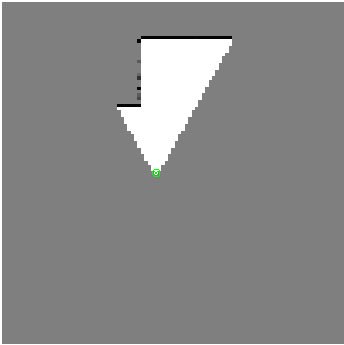
\includegraphics[height=0.4\columnwidth]{Compare_ISM_1.pdf}
	}
	\subfigure[Approximate Model]
		{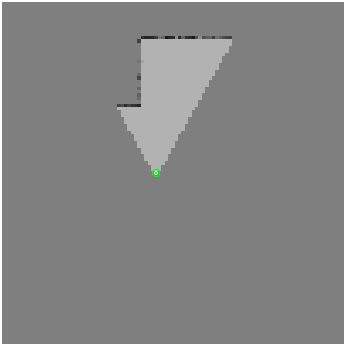
\includegraphics[height=0.4\columnwidth]{Compare_Approx_1.pdf}
	}
}
\centerline{
	\subfigure[Exact Model]
		{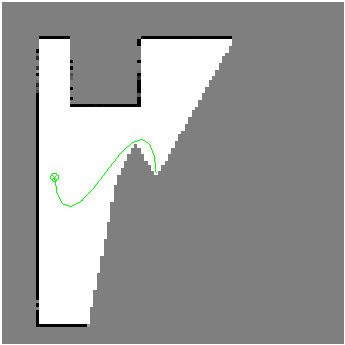
\includegraphics[height=0.4\columnwidth]{Compare_ISM_2.pdf}
	}
	\subfigure[Approximate Model, First Measurement]
		{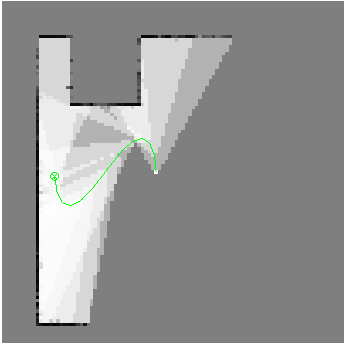
\includegraphics[height=0.4\columnwidth]{Compare_Approx_2.pdf}
	}
}
\centerline{
	\subfigure[Exact Model]
		{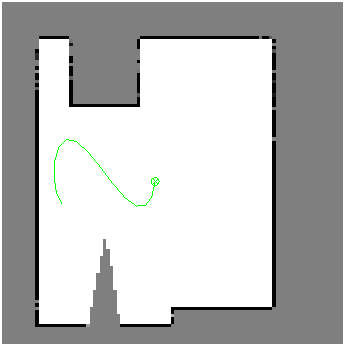
\includegraphics[height=0.4\columnwidth]{Compare_ISM_3.pdf}
	}
	\subfigure[Approximate Model]
		{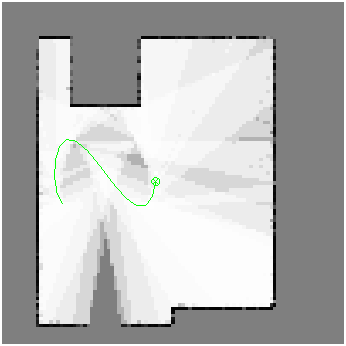
\includegraphics[height=0.4\columnwidth]{Compare_Approx_3.pdf}
	}
}
\centerline{
	\subfigure[Exact Model]
		{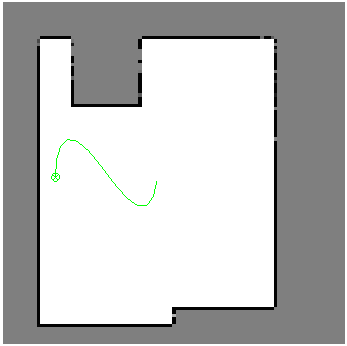
\includegraphics[height=0.4\columnwidth]{Compare_ISM_4.pdf}
	}
	\subfigure[Approximate Model]
		{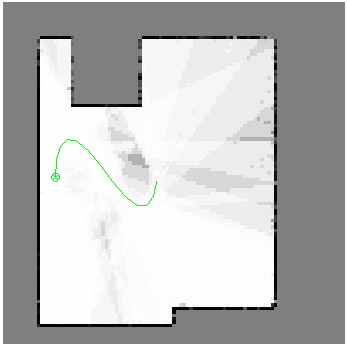
\includegraphics[height=0.4\columnwidth]{Compare_Approx_4.pdf}
	}
}
\centerline{
	\subfigure[Exact Model]
		{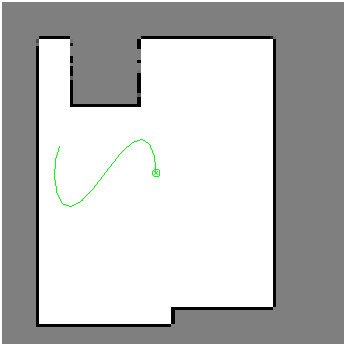
\includegraphics[height=0.4\columnwidth]{Compare_ISM_5.pdf}
	}
	\subfigure[Approximate Model]
		{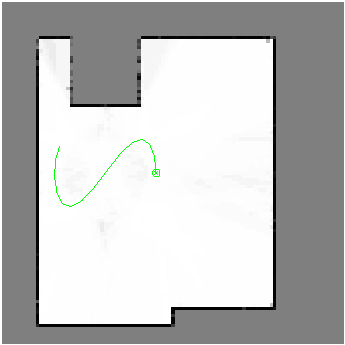
\includegraphics[height=0.4\columnwidth]{Compare_Approx_5.pdf}
	}
}
\caption{The exact inverse sensor model approach proposed in this paper is compared with with an approximate algorithm designed for the Kinect depth sensor. The goal of the occupancy grid mapping algorithms is to update the grid cells from uncertain (grey, $0.5$ occupancy probability) to either occupied (black, $1$ occupancy probability) or free (white, $0$ occupancy probability). Measured cells have occupancy probabilities closer to $0$ or $1$ as more information becomes available, and unmeasured cells remain uncertain. The exact inverse sensor model approach generates a faster and more accurate result.}
\end{figure}

\begin{figure}[h]
\label{fig:NumResOccH}
\centerline{
	\subfigure[Entropy Change (blue: exact model, red: approximation)]
		{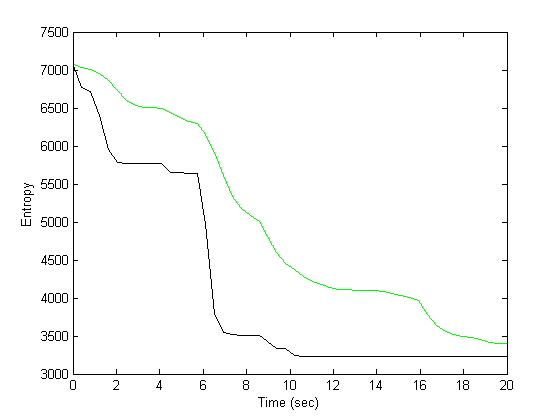
\includegraphics[width=0.8\columnwidth]{EntropyEvolution.png}
	}
}
\centerline{
	\subfigure[Final Exact Model]
		{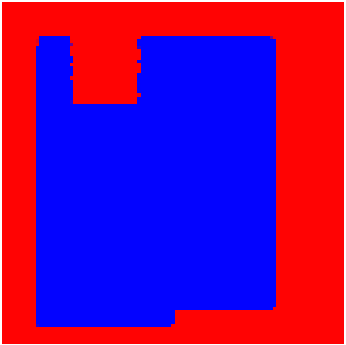
\includegraphics[height=0.4\columnwidth]{Compare_ISM_H.pdf}
	}
	\subfigure[Final Approximate Model]
		{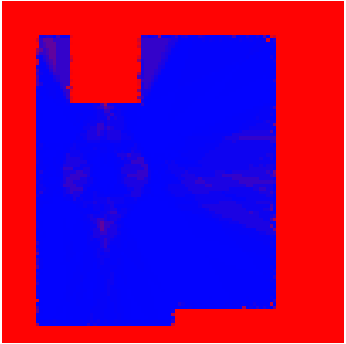
\includegraphics[height=0.4\columnwidth]{Compare_Approx_H.pdf}
	}
}
\caption{Entropy serves as a measure of uncertainty of the occupancy grid, where more blue regions are more certain, and red regions are more uncertain. The uncertainty is always less when the exact solution derived in this paper is applied.}
\end{figure}

The occupancy grids generated by the exact inverse sensor model are yield clearer maps with less uncertainty.
The entropy of the map from the first measurement to the last is less with the exact model, where sudden decreases correspond to sharp turns in the robot motion.
During these turns, the field of view changes greatly, so the information gain from the measurements is large.

\section{Preliminary Experimental Results}
\label{sec:ExpRes}
	% Kinect result

A preliminary experiment shows how the exact inverse sensor model is successfully implemented with the Kinect sensor.
Again, the parameters for the Kinect are obtained from~\cite{KhoElb12}, and the OpenKinect library is used on a Mac computer.
The Kinect sensor faces walls underneath a work desk, where the results are depicted in Figure \ref{fig:ExpRes}

\begin{figure}[h]
\label{fig:ExpRes}
\centerline{
	\subfigure[Test Setup]
		{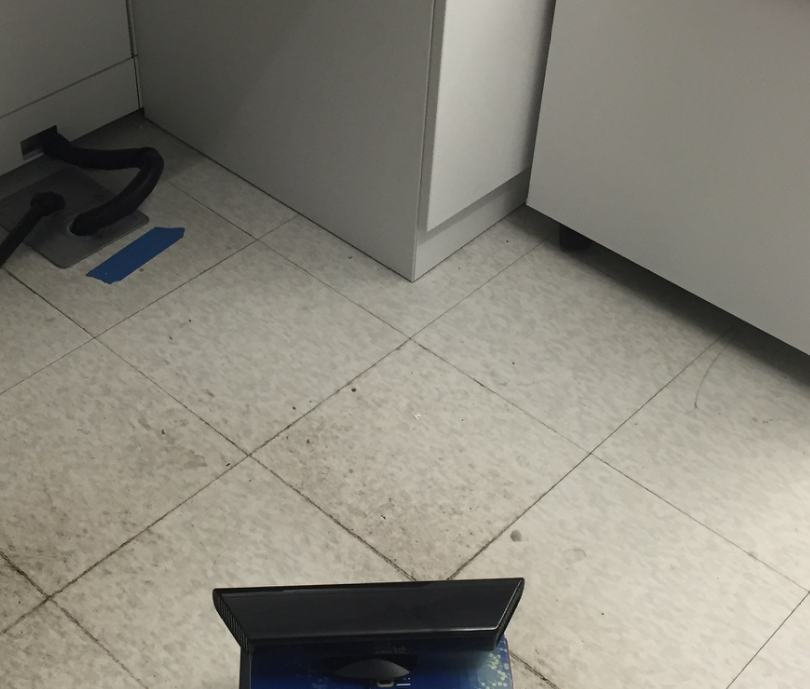
\includegraphics[height=0.3\columnwidth]{TestSetup.png}
	}
	\subfigure[Kinect View]
		{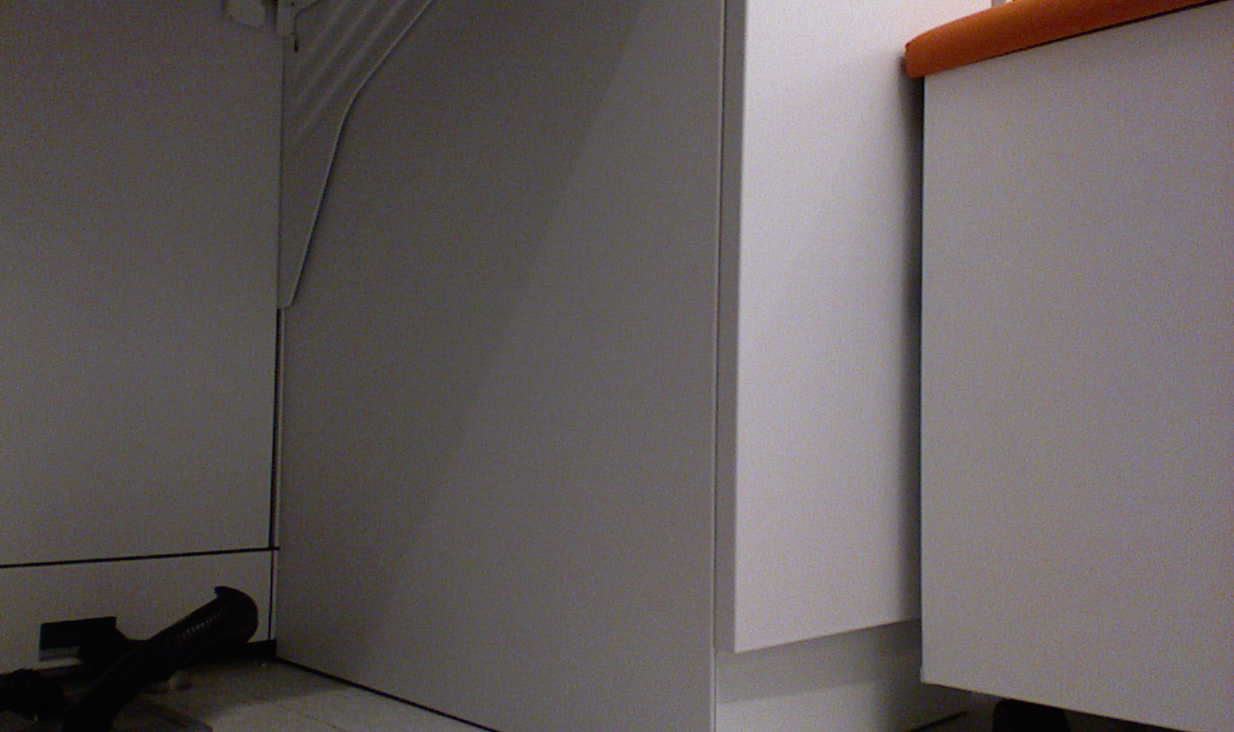
\includegraphics[height=0.3\columnwidth]{KinectView.png}
	}
}
\centerline{
	\subfigure[Exact Model Probabilities]
		{
\includegraphics[height=0.4\columnwidth]{KinectDeskISM.png}
	}
	\hspace*{0.1\columnwidth}
	\subfigure[Approximate Model Probabilities]
		{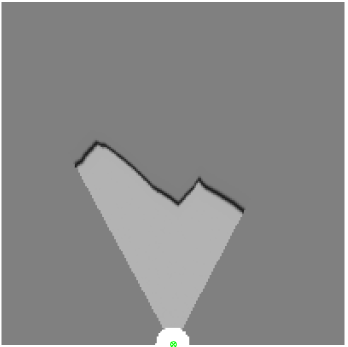
\includegraphics[height=0.4\columnwidth]{KinectDeskApprox.png}
	}
}
\centerline{
	\subfigure[Exact Model Entropies]
		{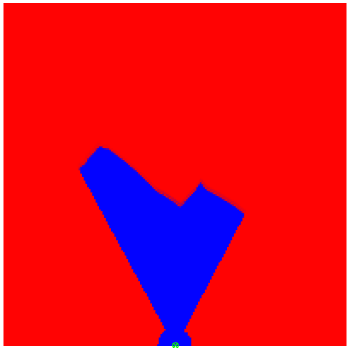
\includegraphics[height=0.4\columnwidth]{KinectDeskISM_H.png}
	}
	\hspace*{0.1\columnwidth}
	\subfigure[Exact Model Entropies]
		{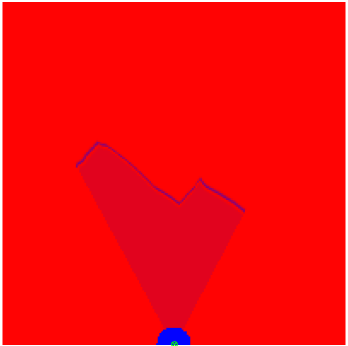
\includegraphics[height=0.4\columnwidth]{KinectDeskApprox_H.png}
	}
}
\caption{The Kinect captures depth measurements of the underside of a metal desk. The measurement scan serves to update two occupancy grid mapping schemes. The proposed approach, based on the the exact solution of the inverse sensor model, provides an update with substantially less uncertainty.}
\end{figure}



%The following challenges were encountered:
%\begin{itemize}
%\item there were some issues with saving depth measurements that are now resolved,
%\item direct distances are not measured (instead from the plane of the sensor to the depth image pixel), and
%\item the conversion between a $16$-bit integer to a distance appears to be nonlinear.
%\end{itemize}
%In short, we used the Kinect camera with a few challenges.
%
%\subsection{Experimental Results}
%
%We compare the occupancy grid mapping approach based on the exact inverse sensor model proposed for this research project with the conventional approach based on \refeqn{ISM_Approx_1} and \refeqn{ISM_Approx_2}.
%The same measurement scan data of the lower part of a desk (Figures 1a and 1b) is used for both algorithms.

The proposed approach uses all the information from the measurement scans accurately. After the first scan, the free space has a substantially lower probability of occupancy. Furthermore, the edges of the objects captured by the Kinect are well defined with the proposed approach with an edge thickness of roughly one or two cells, but two or three cells thick with the conventional approach; of course, the Kinect cannot measure through the metal desks measured, so increases in occupancy probability beyond this edge are not necessary accurate.
Additionally, the decrease in entropy is greater with the proposed approach at $-3487$ compared with just $-557$ with the conventional approach.

\section{Conclusions}

Occupancy grid mapping produces a probabilistic map of occupied space, but each probability is approximated in practice due to the perceived complications of the exact solution.
However, this paper provides an exact solution to this complicated probability problem based using cell occlusion and assuming that the depth measurements have accurate bearing.
The numerical and experimental results show that maps using this exact approach are substantially improved without computational barriers.
	

	
\bibliography{BibSources}
\bibliographystyle{IEEEtran}


\end{document}




\end{document}
